\documentclass[journal,12pt,twocolumn]{IEEEtran}
%
\makeatletter
\makeatother
\usepackage{setspace}
\usepackage{gensymb}
\usepackage{xcolor}
\usepackage{caption}
%\usepackage{stackengine}
%\usepackage{subcaption}
%\doublespacing
\singlespacing



\usepackage{graphicx}
\graphicspath{ {./images}  }
%\usepackage{amssymb}
%\usepackage{relsize}
\usepackage[cmex10]{amsmath}
\usepackage{mathtools}
%\usepackage{amsthm}
\interdisplaylinepenalty=2500
%\savesymbol{iint}
%\usepackage{txfonts}
%\restoresymbol{TXF}{iint}
\usepackage{wasysym}
\usepackage{amsthm}
\usepackage{mathrsfs}
\usepackage{txfonts}
\usepackage{stfloats}
\usepackage{cite}
\usepackage{cases}
\usepackage{mathtools}
\usepackage{subfig}
\usepackage{enumerate}	
\usepackage{enumitem}
\usepackage{amsmath}
%\usepackage{xtab}
\usepackage{longtable}
\usepackage{multirow}
%\usepackage{algorithm}
%\usepackage{algpseudocode}
\usepackage{enumitem}
\usepackage{mathtools}
%\usepackage{iithtlc}
%\usepackage[framemethod=tikz]{mdframed}
\usepackage{listings}
    \usepackage[latin1]{inputenc}                                 %%
    \usepackage{color}                                            %%
    \usepackage{array}                                            %%
    \usepackage{longtable}                                        %%
    \usepackage{calc}                                             %%
    \usepackage{multirow}                                         %%
    \usepackage{hhline}                                           %%
    \usepackage{ifthen}                                           %%
  %optionally (for landscape tables embedded in another document): %%
    \usepackage{lscape}     



%\usepackage{stmaryrd}


%\usepackage{wasysym}
%\newcounter{MYtempeqncnt}
\DeclareMathOperator*{\Res}{Res}
%\renewcommand{\baselinestretch}{4}
%\setcounter{secnumdepth}{4}
\renewcommand\thesection{\arabic{section}}
\renewcommand\thesubsection{\thesection.\arabic{subsection}}
\renewcommand\thesubsubsection{\thesubsection.\arabic{subsubsection}}
%\renewcommand\thesubsubsubsection{\thesubsubsection.\arabic{subsubsubsection}}

%\renewcommand\thesectiondis{\arabic{section}}
%\renewcommand\thesubsectiondis{\thesectiondis.\arabic{subsection}}
%\renewcommand\thesubsubsectiondis{\thesubsectiondis.\arabic{subsubsection}}
%\renewcommand\thesubsubsubsectiondis{\thesubsubsectiondis.\arabic{subsubsubsection}}
% correct bad hyphenation here
\hyphenation{op-tical net-works semi-conduc-tor}

%\lstset{
%language=C,
%frame=single, 
%breaklines=true
%}

%\lstset{
	%%basicstyle=\small\ttfamily\bfseries,
	%%numberstyle=\small\ttfamily,
	%language=Octave,
	%backgroundcolor=\color{white},
	%%frame=single,
	%%keywordstyle=\bfseries,
	%%breaklines=true,
	%%showstringspaces=false,
	%%xleftmargin=-10mm,
	%%aboveskip=-1mm,
	%%belowskip=0mm
%}

%\surroundwithmdframed[width=\columnwidth]{lstlisting}
\def\inputGnumericTable{}                                 %%

\lstset{
%language=python,
frame=single, 
breaklines=true,
columns=fullflexible
}

 

\begin{document}
%

\theoremstyle{definition}
\newtheorem{theorem}{Theorem}[section]
\newtheorem{problem}{Problem}
\newtheorem{proposition}{Proposition}[section]
\newtheorem{lemma}{Lemma}[section]
\newtheorem{corollary}[theorem]{Corollary}
\newtheorem{example}{Example}[section]
\newtheorem{definition}{Definition}[section]
%\newtheorem{algorithm}{Algorithm}[section]
%\newtheorem{cor}{Corollary}
\newcommand{\BEQA}{\begin{eqnarray}}
\newcommand{\EEQA}{\end{eqnarray}}
\newcommand{\define}{\stackrel{\triangle}{=}}

\bibliographystyle{IEEEtran}
%\bibliographystyle{ieeetr}

\providecommand{\nCr}[2]{\,^{#1}C_{#2}} % nCr
\providecommand{\nPr}[2]{\,^{#1}P_{#2}} % nPr
\providecommand{\mbf}{\mathbf}
\providecommand{\pr}[1]{\ensuremath{\Pr\left(#1\right)}}
\providecommand{\qfunc}[1]{\ensuremath{Q\left(#1\right)}}
\providecommand{\sbrak}[1]{\ensuremath{{}\left[#1\right]}}
\providecommand{\lsbrak}[1]{\ensuremath{{}\left[#1\right.}}
\providecommand{\rsbrak}[1]{\ensuremath{{}\left.#1\right]}}
\providecommand{\brak}[1]{\ensuremath{\left(#1\right)}}
\providecommand{\lbrak}[1]{\ensuremath{\left(#1\right.}}
\providecommand{\rbrak}[1]{\ensuremath{\left.#1\right)}}
\providecommand{\cbrak}[1]{\ensuremath{\left\{#1\right\}}}
\providecommand{\lcbrak}[1]{\ensuremath{\left\{#1\right.}}
\providecommand{\rcbrak}[1]{\ensuremath{\left.#1\right\}}}
\theoremstyle{remark}
\newtheorem{rem}{Remark}
\newcommand{\sgn}{\mathop{\mathrm{sgn}}}
\providecommand{\abs}[1]{\left\vert#1\right\vert}
\providecommand{\res}[1]{\Res\displaylimits_{#1}} 
\providecommand{\norm}[1]{\lVert#1\rVert}
\providecommand{\mtx}[1]{\mathbf{#1}}
\providecommand{\mean}[1]{E\left[ #1 \right]}
\providecommand{\fourier}{\overset{\mathcal{F}}{ \rightleftharpoons}}
%\providecommand{\hilbert}{\overset{\mathcal{H}}{ \rightleftharpoons}}
\providecommand{\system}{\overset{\mathcal{H}}{ \longleftrightarrow}}
	%\newcommand{\solution}[2]{\textbf{Solution:}{#1}}
\newcommand{\solution}{\noindent \textbf{Solution: }}
\providecommand{\dec}[2]{\ensuremath{\overset{#1}{\underset{#2}{\gtrless}}}}
\DeclarePairedDelimiter{\ceil}{\lceil}{\rceil}
%\numberwithin{equation}{subsection}
\numberwithin{equation}{section}
%\numberwithin{problem}{subsection}
%\numberwithin{definition}{subsection}
%\makeatletter
%\@addtoreset{figure}{section}
%\makeatother

\let\StandardTheFigure\thefigure
%\renewcommand{\thefigure}{\theproblem.\arabic{figure}}
%\renewcommand{\thefigure}{\thesection}


%\numberwithin{figure}{subsection}

%\numberwithin{equation}{subsection}
%\numberwithin{equation}{section}
%\numberwithin{equation}{problem}
%\numberwithin{problem}{subsection}
%\numberwithin{problem}{section}
%%\numberwithin{definition}{subsection}
%\makeatletter
%\@addtoreset{figure}{problem}
%\makeatother
%\makeatletter
%\@addtoreset{table}{problem}
%\makeatother

\let\StandardTheFigure\thefigure
\let\StandardTheTable\thetable
%%\renewcommand{\thefigure}{\theproblem.\arabic{figure}}
%\renewcommand{\thefigure}{\theproblem}

%%\numberwithin{figure}{section}

%%\numberwithin{figure}{subsection}



\def\putbox#1#2#3{\makebox[0in][l]{\makebox[#1][l]{}\raisebox{\baselineskip}[0in][0in]{\raisebox{#2}[0in][0in]{#3}}}}
     \def\rightbox#1{\makebox[0in][r]{#1}}
     \def\centbox#1{\makebox[0in]{#1}}
     \def\topbox#1{\raisebox{-\baselineskip}[0in][0in]{#1}}
     \def\midbox#1{\raisebox{-0.5\baselineskip}[0in][0in]{#1}}




\title{ 
%	\logo{
Efficient Transmitter Design Techniques in Digital Communication
%	}
}



\author{Theresh Babu Benguluri,Sandeep Kumar Khyalia, Siddharth Maurya, Sai Manasa, Raktim Goswami, Abhishek Bairagi, G V V Sharma$^{*}$% <-this % stops a space
\thanks{*The author is with the Department
of Electrical Engineering, Indian Institute of Technology, Hyderabad
502285 India e-mail:  gadepall@iith.ac.in.}
}


% make the title area
\maketitle

\tableofcontents

\bigskip
%
\begin{abstract}
A brief description of  Efficient Transmitter Design (ETD) techniques is provided. These include Interleaver/Deinterleaver for combating bursty errors, Physical Layer Framing for the efficient detection of Frame starting, and  Pulse Shaping to combat  InterSymbol Interference.
\end{abstract}

%\IEEEpeerreviewmaketitle

\section{Interleaver/Deinterleaver}
For 8PSK, 16APSK, and 32APSK mapping schemes, a
block interleaver  \cite{dvb} is used to mitigate the effects of bursty channel. For Concatenated Channel coding schemes bit interleaving is necessary. The mapped data is serially put as column wise and searially read out row wise. 
%
\begin{figure}[!ht]
\begin{center}
\includegraphics[width=\columnwidth]{/bitinterleaver_8psk}
\end{center}
\caption{Bit Interleaver Structure for 8PSK mapping scheme}
\label{fig:bit8psk}
\end{figure}
Fig. \ref{fig:bit8psk} shows bit interleaving scheme for 8PSK.


Fig. \ref{fig:inter} 
%generated by 
%%
%
shows the BER comparison of 8PSK mapping scheme with  and without interleaver. 
\begin{figure}[!ht]
\begin{center}
\includegraphics[width=\columnwidth]{./figs/Interleaver.eps}
\end{center}
\caption{Bit interleaver for 8PSK}
\label{fig:inter}
\end{figure}


\section{Physical Layer Framing(PLFRAMING)}

PLFRAMING is useful for  specifying the modulation scheme,  code rate and frame characteristics, useful for Frame synchronization at the receiver.  Fig. \ref{fig:splframe} shows the Typical Structure of PLFRAME according to \cite{dvb}.
$SOF$=Starting Of Frame and  $PLSC$=Physical Layer Signalling Code.

%\item In order to form the PLFRAME which is used for receiver synchronization, a header is inserted in the beginning of each frame.
\begin{figure}[!ht]
\begin{center}
\includegraphics[width=\columnwidth]{/pl_framing}
\end{center}
\caption{Structure of PLFRAME.}
\label{fig:splframe}
\end{figure}
%
\subsection{Generation of SOF}
SOF consistutes a fixed sequence $18D2E82_{HEX}$ (length=26 bits) in binary format which is from right to left.

\subsection{Generation of PLSC}
\begin{itemize}
\item Generation of PLSC involes definining 7 symbols and multiplying first 6 symbols with the defined $G$ matrix in \cite{dvb}. First 5 symbols called as MODCOD filed and next 2 symbols as TYPE field.
\item First 5 symbols represents MODCOD which specifies Frame's mapping scheme and code rate.  Fig. \ref{fig:modcod} shows the MODCOD coding for various mapping schemes.
\item Next 2 symbols represents TYPE filed which specifies Frame length and presence and absesnce of pilot fileds.
This is shown in Table \ref{table:type}.
\item  Similarly, Fig. \ref{fig:pls gen} shows the generation of 64 bit using the MODCOD and TYPE bits.
\item  After the generation of PLS code, we will again scramble the PLS Code with the fixed SCR sequence which is defined in \cite{dvb}.
\begin{equation}
PLSC=PLSC \oplus SCR
\end{equation}
 

\end{itemize}
%

%
\begin{table}[!ht]
\begin{center}
{\tiny
\input{./figs/type.tex}
}
\end{center}
\caption{Frame Type}
\label{table:type}
\end{table}

\begin{figure}[!ht]
\begin{center}
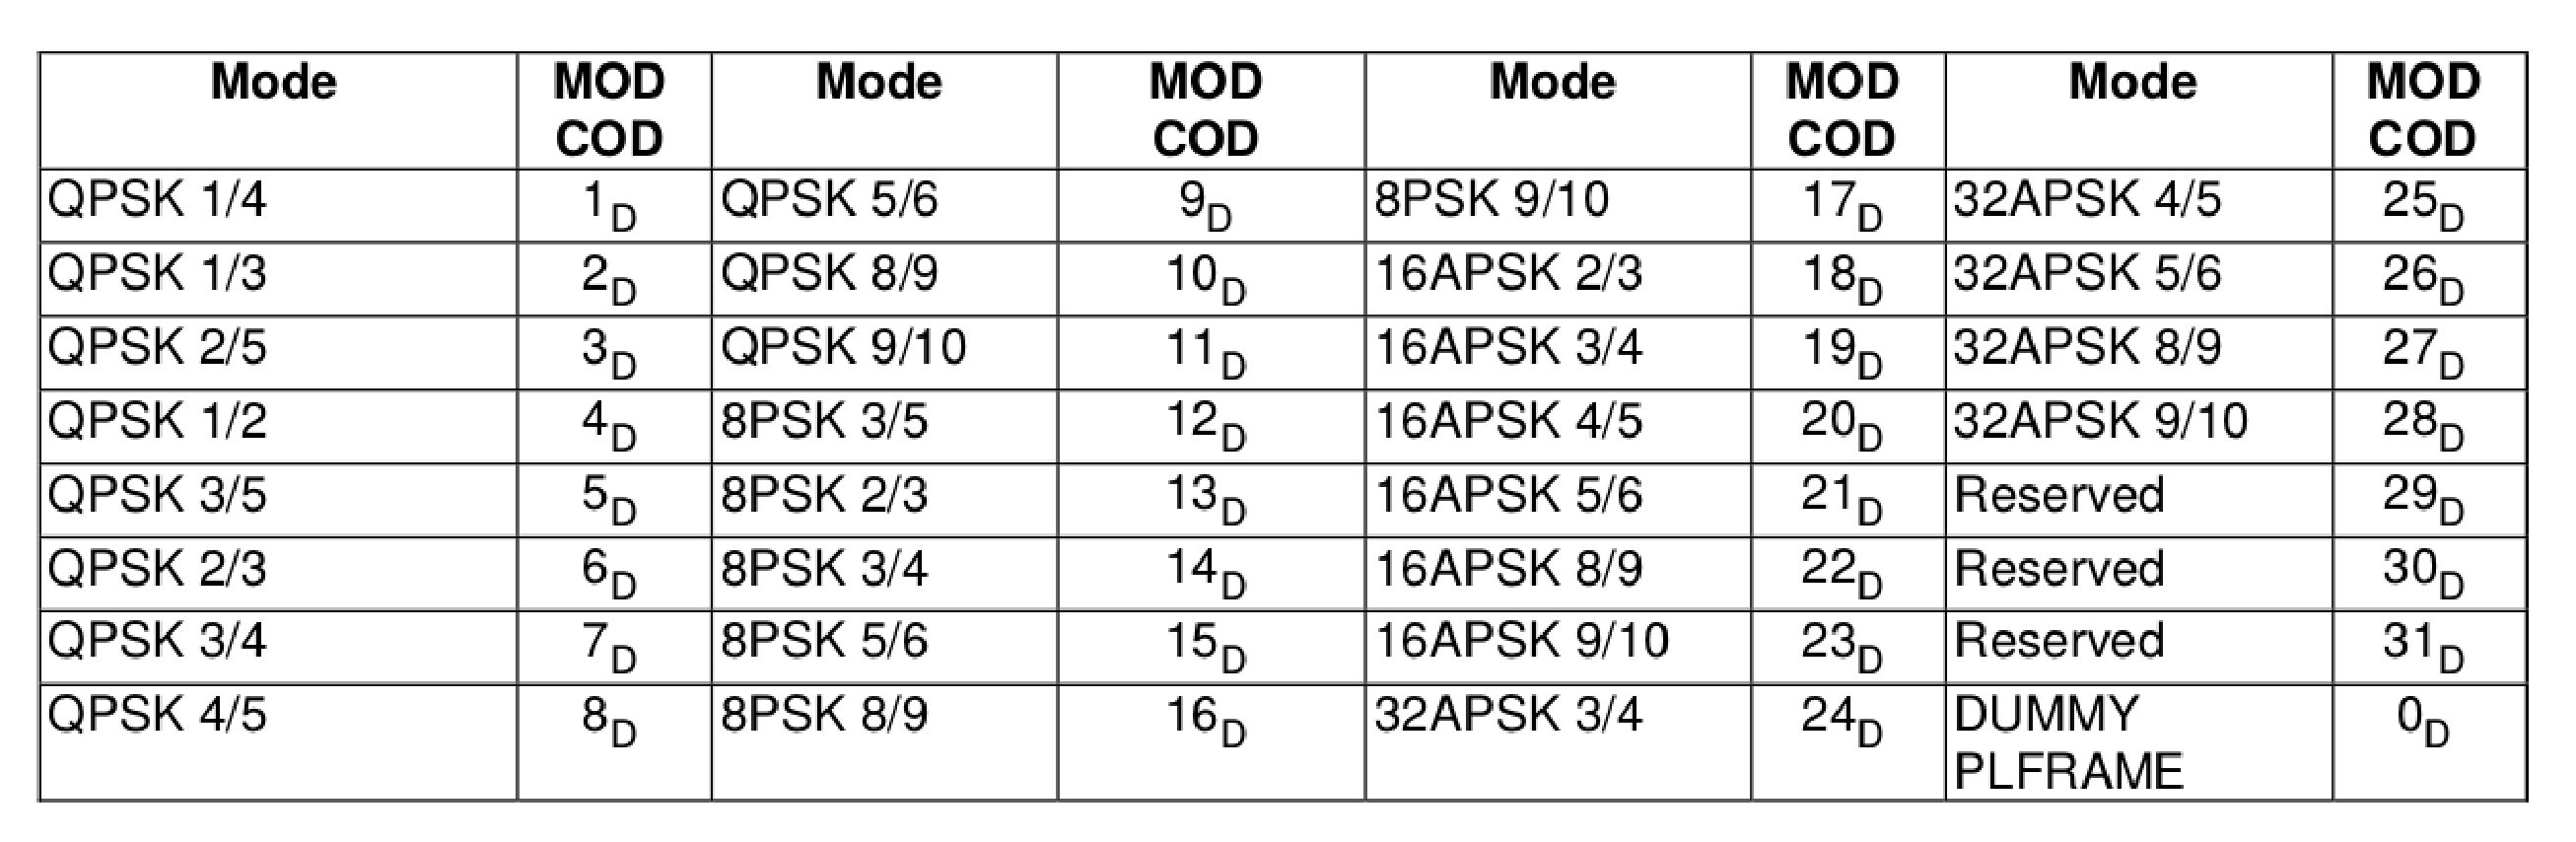
\includegraphics[width=\columnwidth]{/MODCOD}
\end{center}
\caption{MODCOD coding for various mapping schemes. Subscript $D$ denotes decimal e.g. $1_D = 00001$ in binary}
\label{fig:modcod}
\end{figure}
%
%
\begin{figure}[!ht]
\begin{center}
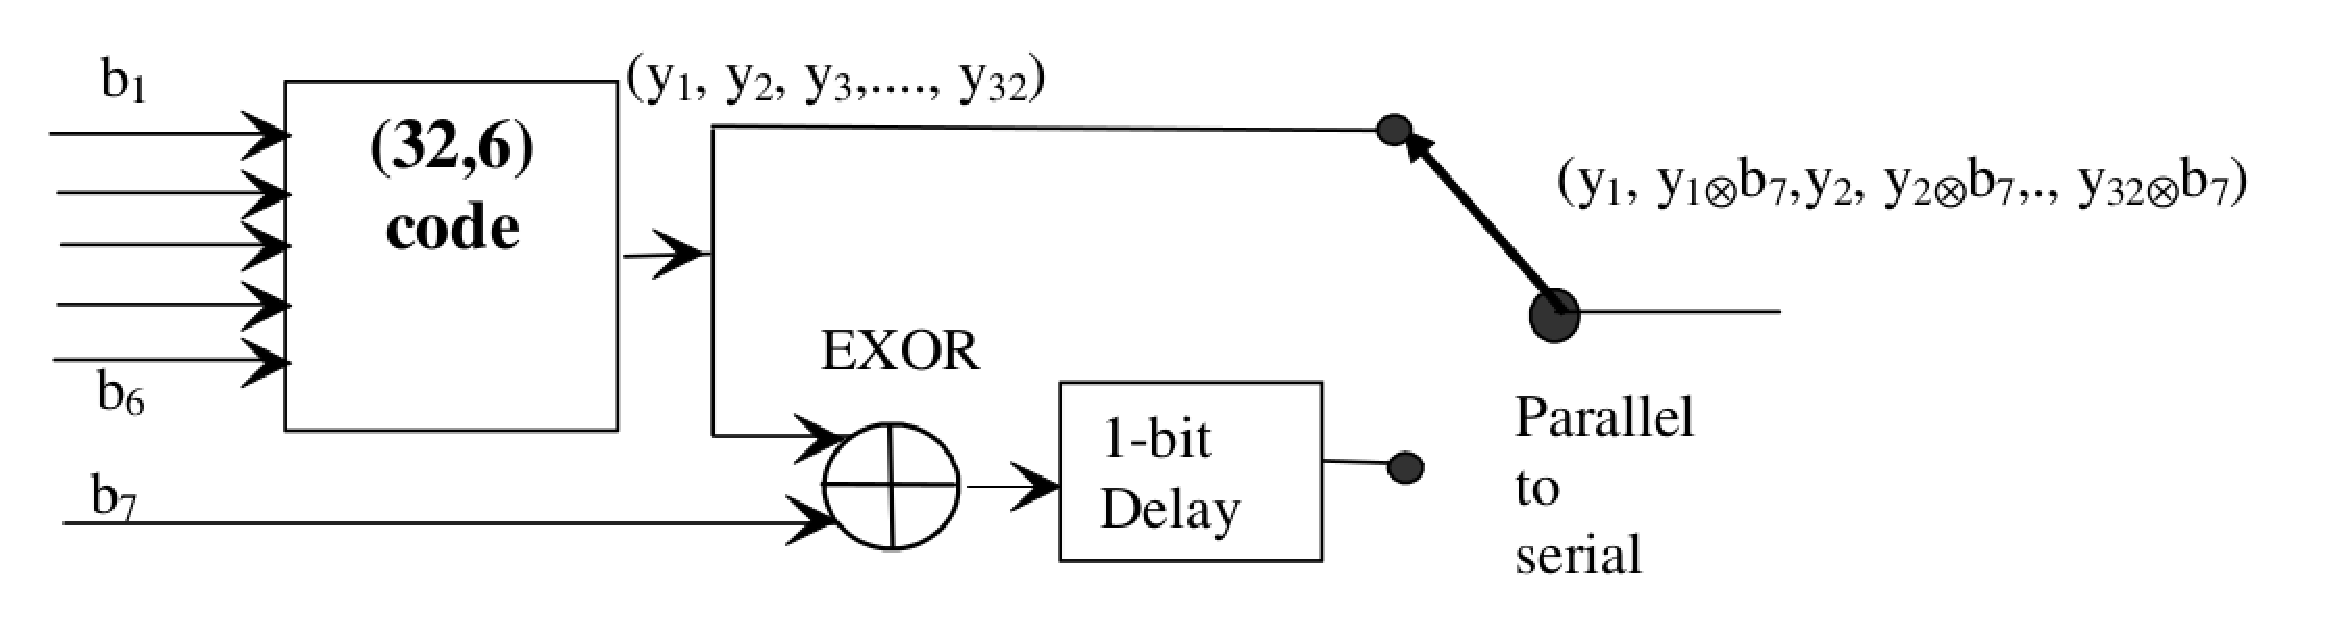
\includegraphics[width=\columnwidth]{/plscode}
\end{center}
\caption{Physical Layer Signalling generation}
\label{fig:pls gen}
\end{figure}
%
\subsection{PLHEADER}
The PLHEADER has SOF (26 symbols) and PLSC (64 symbols) sequences, that are modulated by rotating QPSK by $\frac{\pi}{4}$.  This is also known as  $\frac{\pi}{2}$-BPSK. 
 \begin{align}\label{eq:1}
I_{2i-1}=Q_{2i-1}&=\frac{1}{\sqrt{2}}(1-2y_{2i-1}) \quad i=1,2,\dots,45
\\
\label{eq:2}
I_{2i}=-Q_{2i}&=-\frac{1}{\sqrt{2}}(1-2y_{2i-1}) \quad 1,2\dots,45
\end{align}
%
where $y_i \in \cbrak{0,1},i = 1,\dots,90$.
 
\subsection{Generation of Pilots}
%
%\begin{figure}
%\begin{center}
%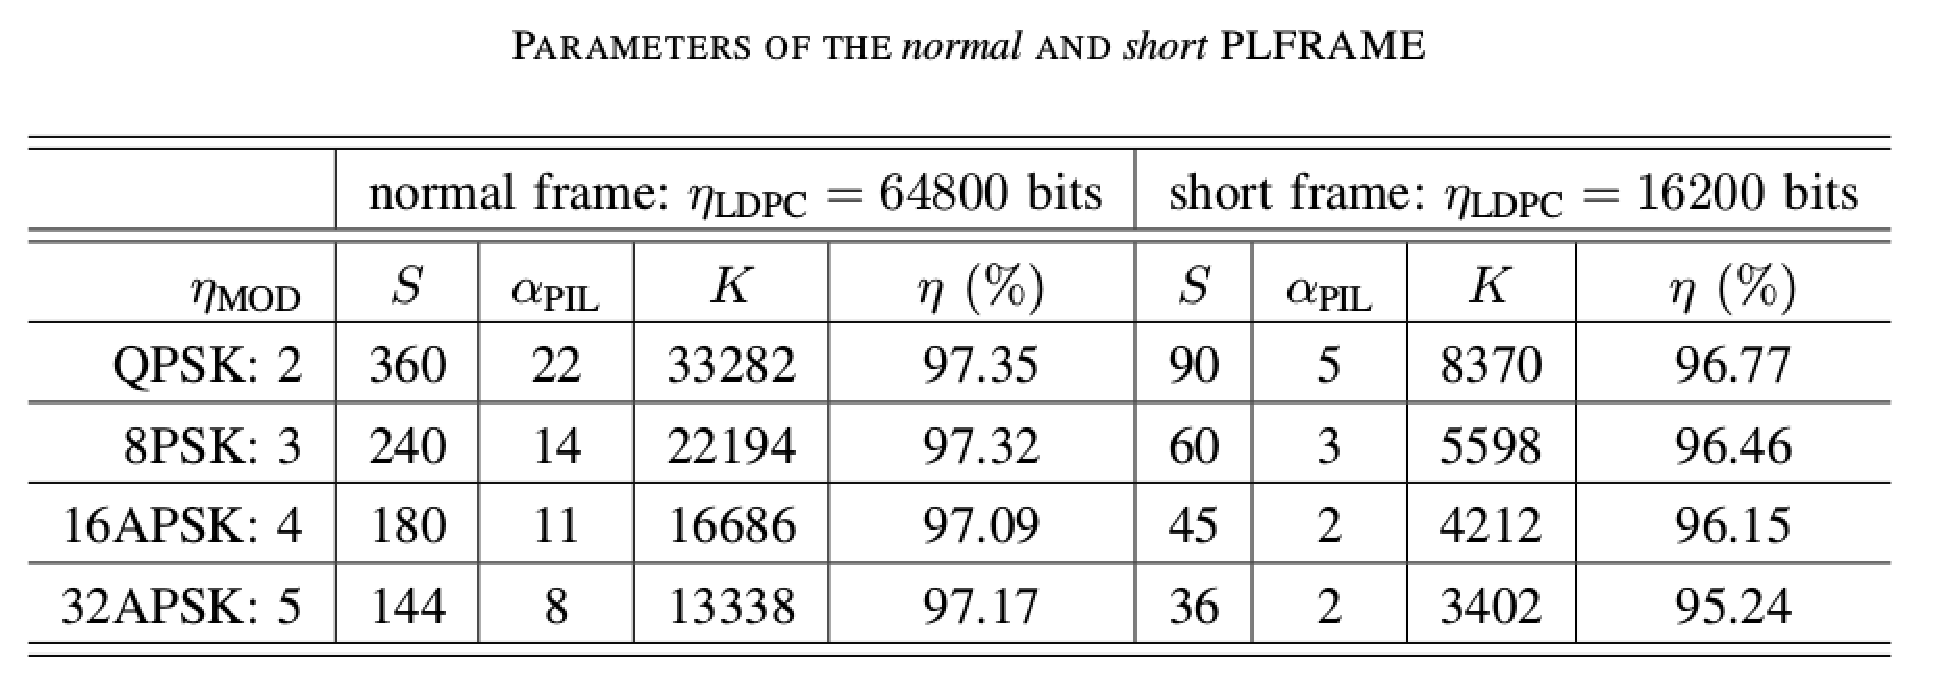
\includegraphics[width=\columnwidth]{/parameters_pl_frame}
%\end{center}
%\caption{paramters of plframe}
%\label{fig:plframe}
%\end{figure}
%%
Pilot block consists of $P=36$ symbols. Each pilot is composed of un-modulated complex symbol.Where, $I=Q=\frac{1}{\sqrt{2}}$ 
%The first pilot block inserted 16 slots after the PLHEADER and next is inserted after the 32 slots and so on.
%\begin{equation}\label{eq:plen}
%K = 
%\begin{cases}
%90\times (S+1)  & \textit{with out pilots}
%\\
%90\times (S+1) + 36\times \alpha_{PIL}  & \textit{with pilots}
%\end{cases}
%\end{equation}
%Where , $\alpha_{PIL}=\left\lfloor \frac{(S-1)}{16} \right\rfloor$.\\
%Eq.\eqref{eq:plen} specifies the total length $K$ of the PLFRAME. Smiliarly, Fig. \ref{fig:plframe} Shows the Parameters of PLFRAME.

% \begin{itemize}
%%\item If pilots are used, then a 36 symbols
%%pilot field is inserted every 16 slots of data symbols. Given that a PLFRAME cannot terminate to a pilot field, the total number of pilot fields is $\alpha_{PIL}=\left\lfloor \frac{(S-1)}{16} \right\rfloor$
%%\item The total length of the PLFRAME in symbols is 
%%\begin{equation}
%%K = 
%%\begin{cases}
%%90\times (S+1)  & \textit{with out pilots}
%%\\
%%90\times (S+1) + 36\times \alpha_{PIL}  & \textit{with pilots}
%%\end{cases}
%%\end{equation}
%%\begin{center}
%%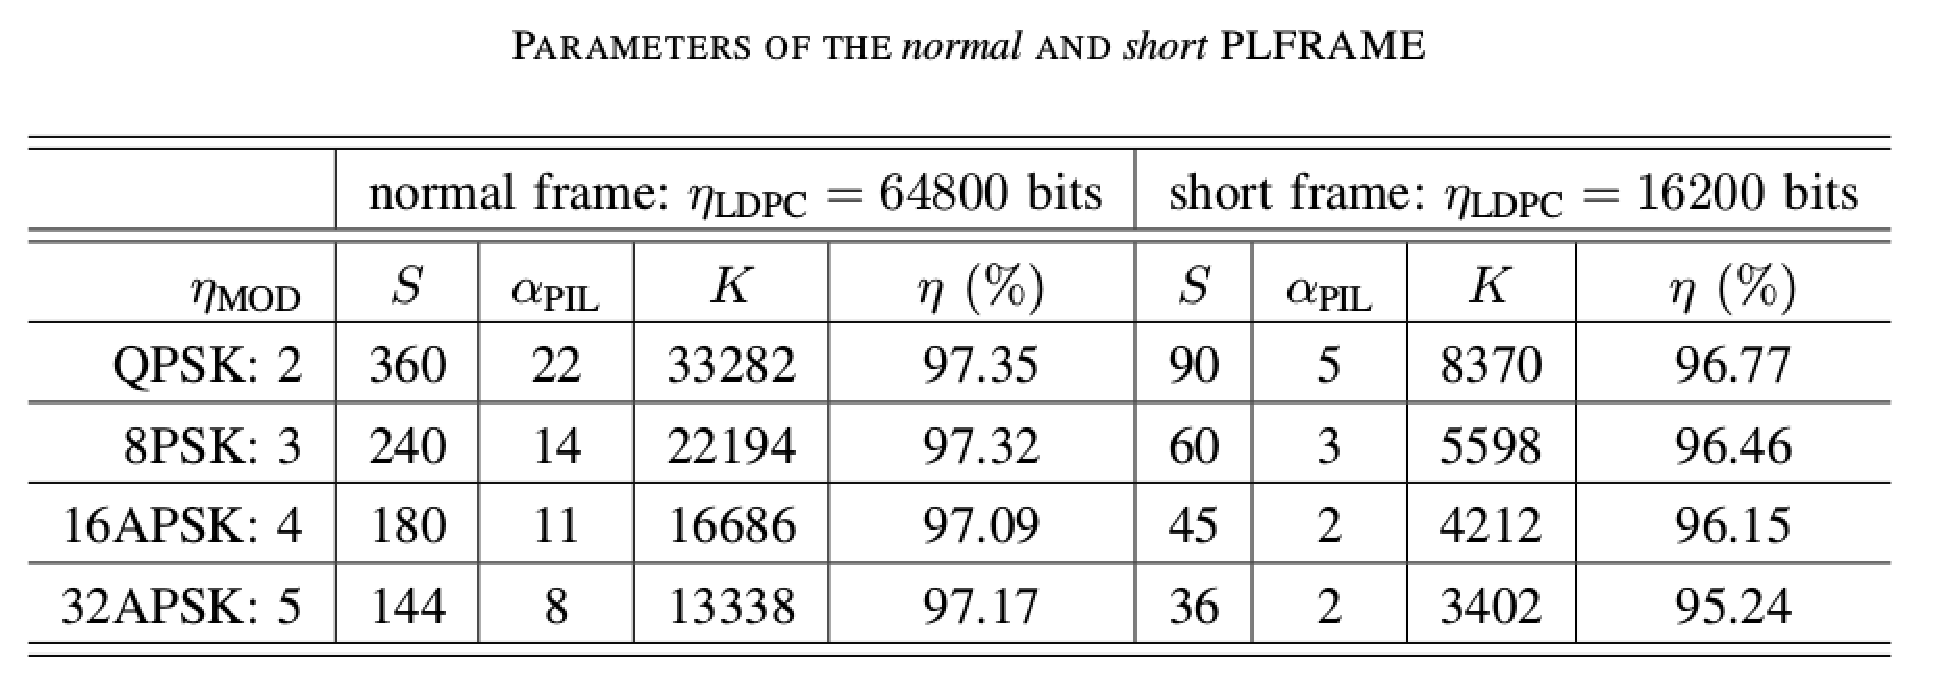
\includegraphics[scale=0.35]{/parameters_pl_frame}
%%\end{center} 
%
%\item The different frame formats,parameters of the normal andshort DVB-S2 frame for all constellation formats were tabulated in above table as  specified in \cite{dvb}
%\end{itemize}
\subsection{PLFRAME Calculations}
PLFRAME calculations are available in Tables \ref{table:splframe1} and \ref{table:splframe2}. 
The PLFRAME length is calculated as
%
\begin{equation}
\label{eq:plength}
L= {SOF}+PLSC+(90*S_{SLOTS})+(36)*P_{SLOTS}
\end{equation}
where,
\begin{equation}
\nonumber
S_{SLOTS}=\frac{N}{90\times\log_2M},P_{SLOTS}=\left\lfloor \frac{(S_{SLOTS}-1)}{16} \right\rfloor
\end{equation}
$N$ = Frame Type(64800/16200 bits),$M$ = Mapping order(4/8/16/32), depending upon the modulation scheme. 


%
\begin{table}[!ht]
\begin{center}
{\tiny
\input{./figs/short.tex}
}
\end{center}
\caption{Short frame details.}
\label{table:splframe1}
\end{table}
%
\begin{table}[!ht]
\begin{center}
{\tiny
\input{./figs/Normal.tex}
}
\end{center}
\caption{Long frame details.}
\label{table:splframe2}
\end{table}

\section{Pulse Shaping}
Let $X_k$ be the modulated symbol in the $k$th time slot.  Then the $m$th sample of the transmitted symbol in the $k$th time slot is
\begin{align}
S_k(m)=h_k(m)* X_k
\end{align}
where $h_k(m), m=1,\dots, M; k=1,\dots,N$ are samples of the pulse shaping filter \cite{dvb}  obtained from
\begin{align}
H(f) =\begin{cases}
1& \abs{f}<f_N(1-\alpha)\\
\cbrak{\frac{1}{2}+\frac{1}{2}\sin \frac{\pi}{2}\sbrak{\frac{f_N-\abs{f}}{\alpha}}}^{\frac{1}{2}}&\abs{f}=f_N(1-\alpha)\\
0&\abs{f}>f_N(1+\alpha)
\end{cases}
\label{eq:pulse_shape}
\end{align}
%
where $f_N$ is the Nyquist frequency and $\alpha = 0.35, 0.25$ or $0.2$.
Let the $m$th received sample in the  $k$th time slot be $Y_k(m)$. At the Receiver, the symbol to be demodulated is then obtained as
\begin{align}
Y_k(m)*h_k(M-m)
\end{align}
The following code plots Fig. \ref{fig:pulseshaping} using pulse shaping.
\begin{lstlisting}
wget https://github.com/gadepall/EE5837/raw/master/ETD/codes/pulse_shaping_qpsk_final.py
\end{lstlisting}
\begin{figure}[!ht]
\begin{center}
\includegraphics[width=\columnwidth]{./figs/pulseshaping}
\end{center}
\caption{SER comparison for QPSK with and without the pulse in \eqref{eq:pulse_shape}.}
\label{fig:pulseshaping}
\end{figure}

%\begin{multline}
%=H_k(m)* X_k + V_k(m) 
%\\
%\end{multline}
%where $H_k(m)$ represents the pulse shape and $V_k(m) \sim \mathcal{N}\brak{0,\sigma^2} $.



%\begin{itemize}
%\item After randomization, the signals shall be square root raised cosine filtered. The roll-off factor shall be $\alpha$ = 0,35, 0,25and 0,20, depending on the service requirements.
%\item Suitable $H(f)$ will be choosen from the \cite{dvb}.
%\begin{align}
%H(f) =\begin{cases}
%1& \abs{f}<f_N(1-\alpha)\\
%\cbrak{\frac{1}{2}+\frac{1}{2}\sin \frac{\pi}{2}\sbrak{\frac{f_N-\abs{f}}{\alpha}}}^{\frac{1}{2}}&\abs{f}=f_N(1-\alpha)\\
%0&\abs{f}>f_N(1-\alpha)
%\end{cases}
%\end{align}
%
%\end{itemize}

\bibliography{IEEEabrv,others.bib}
\end{document}

